%!TEX root = ../thesis.tex

本章では, 先行研究を基にした提案手法をデータの収集方法, 訓練時, テスト時の3節に分けて紹介する. 
\section{データの収集方法}
\figref{Fig:collect-data}にデータの収集方法を示す. 赤色の線である目標経路から±0.1, ±0.2, ±0.4, ±0.6, ±0.8, ±1.0, ±1.5, ±2.0, ±3.0m離れた座標にロボットを配置する. そして, その座標ごとに目標経路に沿った向きを基準として±5度傾けて画像とルールベース制御器によるナビゲーションの出力である角速度を収集する. これを\figref{Fig:willow-garage}に示すコースで一周行う. 

\vspace{10mm}

\begin{figure}[h]
  \centering
  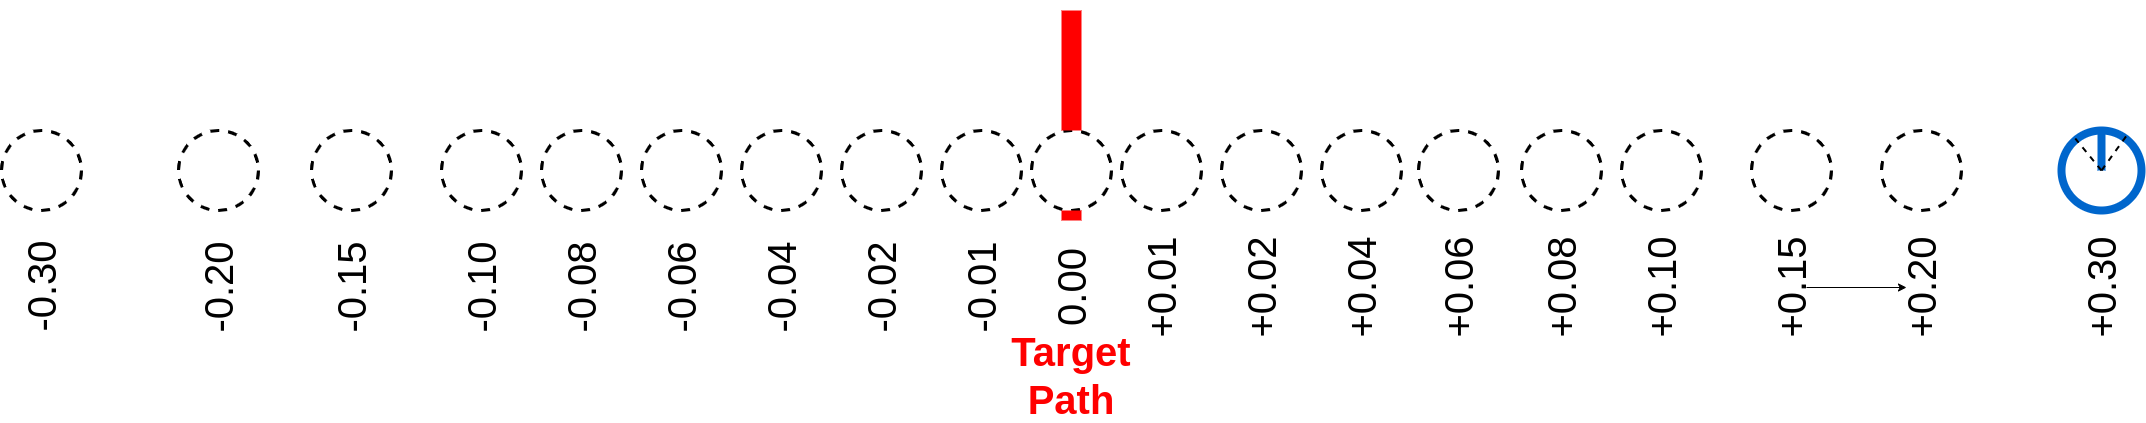
\includegraphics[keepaspectratio, scale=0.18]{images/collect-data.png}
  \caption{Method of collecting data around the target route}
  \label{Fig:collect-data}
  \end{figure}

\newpage
\begin{figure}[h]
  \centering
  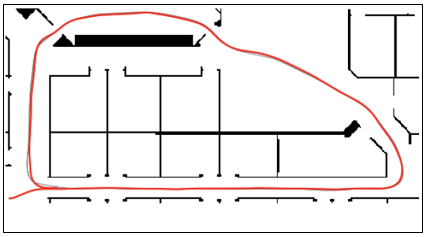
\includegraphics[keepaspectratio, scale=0.5]{images/willow-garage.png}
  \caption{Course to collect data}
  \label{Fig:willow-garage}
  \end{figure}